\documentclass[12pt]{report}
\usepackage[utf8]{inputenc}
\usepackage{graphicx}
\usepackage{float}
\usepackage[hidelinks]{hyperref}
\usepackage[spanish]{babel}
\usepackage{biblatex}
\addbibresource{references.bib}
\graphicspath{ {images/} }

\title{
    {Desarrollo de videojuegos para un solo dev}\\
    {\large Universidad de Cuyo}\\
}
\author{Franco Sorbello}
\date{Day Month Year}

\begin{document}
\maketitle
\tableofcontents
\chapter{Introducción}
\section{Motivación}

\par La industria de los videojuegos es destacada por su constante crecimiento y rentabilidad. No solo esto, si no que requiere una mano de obra altamente especializada. Programadores, músicos, artistas y escritores forman equipos para crear obras de arte interactivas. Sin embargo, la gestión de equipos tan diversos y la coordinación de múltiples tareas presenta un desafío considerable a la hora de llevar a cabo un proyecto de desarrollo de videojuegos.
\bigbreak
Este desafío aumenta al desarrollar un juego desde la perspectiva de un solo dev, es decir que el trabajo es llevado a cabo por una sola persona. El trabajo que comúnmente caería en otros miembros del equipo, como artistas o músicos, pasa a ser responsabilidad del desarrollador. Es por esto que este trabajo busca una metodología que permita llevar a cabo ese proceso de forma ágil y accesible.
\bigbreak
En general, en videojuegos no parece haber una línea clara a la hora de definir una metodología de trabajo. Por un lado, las metodologías ágiles, explicadas en el capítulo 2, parecen ser populares en el desarrollo de videojuegos. En 2013, Koutonen and Leppänen entrevistaron a 20 estudios finlandeses, donde todos menos uno indicaron que aplicaban Agile en al menos una de las fases de desarrollo \cite{koutonenHowAreAgile2013}.
En 2016, Politowski et al. entrevistaron a 58 desarrolladores brasileños y también encontraron un alto uso de metodologías ágiles \cite{politowskiSoftwareEngineeringProcesses2016}.
De forma similar, en 2021 McKenzie et al. entrevistaron a 8 estudios de Nueva Zelanda, los cuales indican utilizar alguna estrategia ágil, como Scrum o Kanban \cite{mckenzieAgileNotAgile2021}.
Finalmente, en 2025 Saarentaurus entrevistó a 5 productores de empresas de videojuegos finlandesas, y todos indicaron que utilizaban Agile en sus proyectos \cite{saarentausAgileScrumMethods2025}.
Estos productores trabajaban en empresas distintas, y todos tenían más de 5 años de experiencia en la industria. Cabe destacar que el estudio se realizó en empresas con más de 100 empleados \cite{saarentausAgileScrumMethods2025}.
\break
Si bien el tamaño de las muestras en cada estudio es pequeño, se puede notar que a lo largo de los años las metodologías ágiles han mantenido un nivel de relevancia en el desarrollo de videojuegos
\bigbreak
Otro fenómeno común al desarrollo es que los estudios terminen utilizando lo que se conoce como metodologías ad-hoc, que consiste en editar otros métodos de desarrollo con el objetivo de ajustarlas a las necesidades de la empresa. McKenzie et al. destacó que si bien los desarrolladores entrevistados indican usar metodologías ágiles, la mayoría realizan modificaciones a Scrum, como eliminar ciertas prácticas, o cambiar la duración de otras \cite{mckenzieAgileNotAgile2021}.
Estos cambios se deben a que es necesario adaptar Scrum a las particularidades del desarrollo de videojuegos \cite{mckenzieAgileNotAgile2021,bartoszScrumVideoGames2023}.
Como se explicó anteriormente, en la creación de un juego participan personas de áreas totalmente distintas, desde programación hasta música. Además, como los juegos son un producto de entretenimiento, uno de los requerimientos del software es que sea “divertido”. Esto es un problema a la hora de planificar ya que es difícil establecer objetivos basados en algo tan subjetivo como la diversión \cite{mckenzieAgileNotAgile2021,bartoszScrumVideoGames2023}. Es por esto que las empresas terminan realizando cambios a la metodología que adoptan.
\bigbreak
A esto se suma que algunos autores han propuesto metodologías específicas para el desarrollo de videojuegos. En 2024, Widjaja et al. desarrollaron un juego utilizando la metodología propuesta por Ramadan y Widyani \cite{widjajaUtilizingGameDevelopment2024}. Este sistema propone un modelo similar a modelos evolutivos pero incluye criterios de calidad relacionados con crear un producto “divertido” \cite{ramadanGameDevelopmentLife2013}. De forma similar, Harman propone un framework que separa distintas etapas del desarrollo en un método de cascada, y luego utiliza conceptos de metodologías ágiles en algunas de ellas \cite{harmanDevelopmentMethodologiesGame2023}.
\bigbreak
Hay un tercer grupo de desarrolladores que no es mencionado en los estudios anteriormente nombrados; los solo devs, o equipos pequeños (2-5 personas). La dinámica de desarrollo cambia debido a la poca cantidad de personas involucradas. No hay mucha investigación al respecto, pero de las fuentes obtenidas se puede observar el uso de metodologías ad-hoc, lo cual es congruente con lo mencionado anteriormente. Similar a Radaman, Widyani y Harman, Anderson separa el desarrollo en etapas de un método en cascada. Además, utiliza Kanban para organizar las tareas \cite{andersonProductionPointHow2023}. Robinson-Yu presenta una idea parecida, con el agregado de utilizar una versión simplificada de Scrum para llevar a cabo sus tareas \cite{gamedevelopersconferenceCraftingTinyOpen2020}.
\bigbreak
En este documento se estudian estas 3 vertientes, con el objetivo de formar una metodología que permita desarrollar un juego como solo dev, tomando los elementos que se consideren útiles y eliminando los que dificulten el trabajo.





\section{Objetivos}
El objetivo de este trabajo es encontrar un proceso de trabajo que permita desarrollar un videojuego como un solo dev. Para ello, se investigan herramientas y metodologías provenientes tanto del software tradicional como de los videojuegos.
\bigbreak
Los objetivos particulares derivados de lo anterior son:
\begin{enumerate}    
    \item Estudiar los frameworks utilizados en el software tradicional.
    \item Estudiar los frameworks específicos del desarrollo de videojuegos.
    \item Con la información anterior, crear un videojuego. Documentar el proceso, notando fortalezas y debilidades de la metodología elegida
\end{enumerate}






\chapter{Ingeniería de software}
\section{Definición de software}
En la actualidad, el software es una institución transversal al funcionamiento del mundo. Los gobiernos y otras entidades públicas son manejados mediante computadoras. Tanto el sector público como el privado utilizan la tecnología para automatizar la mayoría de industrias. Inclusive el arte es afectado por el software, con programas que asisten a la creación de música, pintura o video, entre otros \cite{sommervilleIngenieriaSoftware9a2011}.
\bigbreak
Formalmente, un software es definido como un “conjunto de programas de cómputo, procedimientos, reglas, documentación y datos asociados, que forman parte de las operaciones de un sistema de computación” \cite{alarconaldanaMetodologiaParaDesarrollo2020}. Sin embargo, el software tiene una serie de características que dificultan una definición única.
\begin{enumerate}
    \item El software se desarrolla o modifica con intelecto: los programas son productos intangibles, y por lo tanto no están regidos por procesos de fabricación comunes \cite{sommervilleIngenieriaSoftware9a2011,pressmanIngenieriaSoftwareEnfoque2013}
    \item El software no se desgasta: el software no es susceptible a las condiciones físicas que, por ejemplo, producen un desgaste en la usabilidad de un producto. Sin embargo, el software sí se deteriora. A lo largo de su desarrollo, el software sufre cambios que producen fallas. Estos cambios suelen traer mayor complejidad, por lo que estos errores aumenten en cantidad y dificultad \cite{sommervilleIngenieriaSoftware9a2011,pressmanIngenieriaSoftwareEnfoque2013}.
    \item El software se construye modularmente: a medida que una disciplina de la ingeniería avanza, se crean componentes estándar para utilizar en el diseño. Por ejemplo, tornillos, o circuitos integrados que están preconstruidos. Algo similar sucede en el software, donde se crean componentes reutilizables en otros programas, y sirven como ladrillos para construir nuevos programas \cite{sommervilleIngenieriaSoftware9a2011,pressmanIngenieriaSoftwareEnfoque2013}.
\end{enumerate}
\bigbreak
Por otro lado, a lo largo de los años han aparecido distintos tipos de software que satisfacen mercados variados. Se pueden encontrar:
\begin{itemize}
    \item \textbf{Software de sistemas}, que dan servicios a otros programas. Algunos ejemplos son compiladores, software de redes, o sistemas operativos \cite{pressmanIngenieriaSoftwareEnfoque2013}.
    \item \textbf{Aplicaciones independientes}, programas aislados que resuelven una necesidad específica y corren localmente en una PC \cite{sommervilleIngenieriaSoftware9a2011,pressmanIngenieriaSoftwareEnfoque2013}.
    \item \textbf{Software de ingeniería y ciencias}, que ayudan en procesos de investigación, simulación o cálculos matemáticos complejos.
    \item \textbf{Software embebido}, pensado para controlar dispositivos de hardware pequeños. Un ejemplo sería el panel de un microondas.
    \item \textbf{Aplicaciones web}, distinguidas por su fácil acceso, por lo general desde un navegador web.
    \item \textbf{Software de inteligencia artificial}, que utilizan algoritmos complejos para analizar grandes cantidades de datos.
\end{itemize}
\par
Esta tesina se enfoca en el videojuego, un arte nacido específicamente del software, y que no es capaz de existir fuera de él. Un aspecto interesante de ellos es que se ajustan a varios modelos. Pueden ser programas aislados, o tener conexión a servidores. En algunos casos, se pueden jugar desde un navegador web \cite{PhaserFastFun}. Inclusive, algunos motores gráficos se utilizan para simulación y entrenamiento de inteligencia artificial \cite{MLAgentsOverviewML,UnrealEngineAdvanced}.

\section{Metodologías} %TODO: cambiar titulo
\par A medida que la tecnología avanza, el software se vuelve cada vez más complejo, con programas que requieren múltiples funcionalidades, integración con otros sistemas y constante cambio para ajustarse a las necesidades de los clientes.
\par Esta complejidad plantea desafíos a la hora de crear y mantener un software. Para abordar esta problemática, surgieron las metodologías de desarrollo de software (SDLC en inglés). El objetivo principal de las SDLC es simplificar el proceso de desarrollo y mantenimiento de software. Esto se logra mediante el uso de frameworks que definen una estructura clara para cada fase del ciclo de vida del software, desde la planificación inicial y el diseño, hasta la implementación, las pruebas, el despliegue y el mantenimiento a largo plazo \cite{sStudySoftwareDevelopment2017,rupareliaSoftwareDevelopmentLifecycle2010}. Generalmente, las SDLC comparten una serie de fases comunes a todos los frameworks.

\begin{enumerate}
    \item \textbf{Planning}: En esta etapa se comunica con el cliente y se establece la viabilidad y costo de desarrollar el software \cite{sStudySoftwareDevelopment2017,dwivediComparativeStudyVarious2022} . El objetivo es evaluar los objetivos de los participantes y reunir los requerimientos que ayuden a definir el producto final \cite{pressmanIngenieriaSoftwareEnfoque2013}
    \item \textbf{Definición de requerimientos}: En este paso se ahonda en las necesidades del cliente, mediante conversaciones y entrevistas con los consumidores y dueños del software. Luego, el equipo analiza cada requerimiento y evalúa las posibles ventajas y desventajas de llevarlo a cabo, además de las posibles dificultades técnicas y de diseño que traiga \cite{pressmanIngenieriaSoftwareEnfoque2013,sStudySoftwareDevelopment2017,dwivediComparativeStudyVarious2022}.
    \item \textbf{Diseño}: Las especificaciones del paso anterior se utilizan para plantear el diseño del software. El objetivo es crear un plan que guíe el desarrollo \cite{pressmanIngenieriaSoftwareEnfoque2013,sStudySoftwareDevelopment2017,dwivediComparativeStudyVarious2022}. En ciertas metodologías, este plan es final, e indica los objetivos a cumplir, los tiempos en los que se llevarán a cabo, y las entregas del software.
    \item \textbf{Desarrollo}: Como el nombre lo indica, esta etapa consiste en la creación de código y assets requeridos para el proyecto \cite{pressmanIngenieriaSoftwareEnfoque2013,sStudySoftwareDevelopment2017,dwivediComparativeStudyVarious2022}. Algunas herramientas comunes son lenguajes de programación como C\# o Javascript, además de debuggers\footnote{debugger:programa utilizado para detectar errores en un software.} y otras herramientas de testing \footnote{testing: proceso de detectar errores en un software.}.
    \item \textbf{Testing}: Se crea un ambiente de testing, donde los desarrolladores buscan errores en el software y sus distintas funcionalidades \cite{pressmanIngenieriaSoftwareEnfoque2013,sStudySoftwareDevelopment2017,dwivediComparativeStudyVarious2022}.
    \item \textbf{Deployment}: El software se vuelve accesible para los clientes. En algunos casos, se provee entrenamiento a los usuarios \cite{pressmanIngenieriaSoftwareEnfoque2013,sStudySoftwareDevelopment2017,dwivediComparativeStudyVarious2022}.
    \item \textbf{Mantenimiento}: Se continúa dando soporte al software a medida que es utilizado por los clientes \cite{pressmanIngenieriaSoftwareEnfoque2013,sStudySoftwareDevelopment2017,dwivediComparativeStudyVarious2022}.
\end{enumerate}


\section{Modelos lineales}
Los modelos lineales surgieron con el propósito de estructurar el desarrollo de software, que inicialmente carecía de orden. Constituyen la base de la ingeniería de software \cite{pressmanIngenieriaSoftwareEnfoque2013}. En ellos, el desarrollo se separa en etapas que se llevan a cabo de forma secuencial. Si bien en el presente se favorecen sistemas más interactivos, los modelos lineales son la base en la que se construye el desarrollo del software.
%
%
\subsection{Modelo en cascada}
\par El modelo en cascada es el más básico de las SDLC. En este modelo, se avanza por cada etapa secuencialmente, desde la concepción del producto hasta su entrega \cite{pressmanIngenieriaSoftwareEnfoque2013,sStudySoftwareDevelopment2017,dwivediComparativeStudyVarious2022}. Cada etapa es considerada un módulo independiente, y sólo se avanza cuando se ha completado \cite{dwivediComparativeStudyVarious2022}.
\par Durante la primera etapa, se establecen los requerimientos a completar, además de un plan de acción que engloba a todas las actividades de cada módulo. Cada fase genera uno o más documentos que permiten avanzar a la siguiente fase una vez que son aprobados \cite{sommervilleIngenieriaSoftware9a2011}. Este proceso se continúa hasta completar el software.
%
\begin{figure}[h]
  \centering
  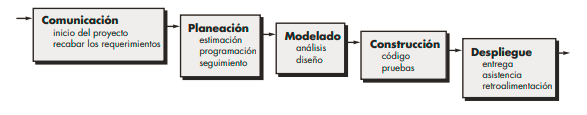
\includegraphics[scale=0.5]{image3.png}
  \caption{Modelo en cascada. Extraída de \cite{pressmanIngenieriaSoftwareEnfoque2013}.}
  \label{fig:x Modelo en cascada}
\end{figure}
%
\par Este modelo es el más antiguo de la ingeniería del software, ideado inicialmente en 1956 por el autor Herbert Bennington y luego modificado por Winston Royce en 1970 [17].
El modelo original, provisto por Bennington, recomendaba desarrollar el software en etapas separadas. Royce luego reconoció que en situaciones reales podrían aparecer dificultades inesperadas, por lo que su versión de cascada añade puntos de retorno en cada etapa, en caso de que sea necesario revisitar un estado anterior \cite{rupareliaSoftwareDevelopmentLifecycle2010,royceManagingDevelopmentLarge1970}. Sin embargo, la mayoría de las organizaciones aplican este modelo de forma estrictamente lineal \cite{pressmanIngenieriaSoftwareEnfoque2013}.
\begin{figure}[h]
  \centering
  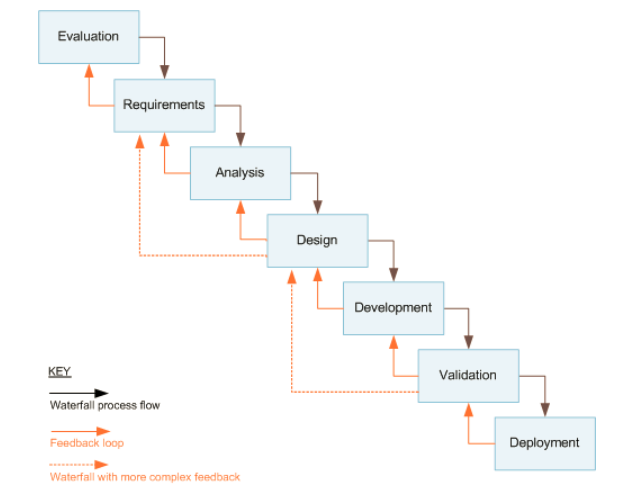
\includegraphics[scale=0.5]{image2.png}
  \caption{Modelo en cascada propuesto por Bennington. Extraída de \cite{rupareliaSoftwareDevelopmentLifecycle2010}.}
  \label{fig:x Modelo en cascada propuesto por Bennington}
\end{figure}
\subsubsection{Ventajas}
\begin{itemize}
  \item Útil para proyectos pequeños donde haya fases claramente definidas.
  \item Cada fase genera un producto entregable.
  \item Documentación extensa de los procesos y resultados.
\end{itemize}
\subsubsection{Desventajas}
\begin{itemize}
  \item Mucha resistencia al cambio, hace que sea difícil implementar en situaciones reales donde los requisitos varían constantemente.
  \item Los requerimientos se establecen al principio y no se pueden cambiar.
  \item No se obtiene un producto funcional hasta el final del proceso.
\end{itemize}
%
%
\subsection{Modelo en V}
\par El modelo en V, también conocido como el modelo de validación y verificación, es una variación del modelo en cascada \cite{rupareliaSoftwareDevelopmentLifecycle2010} donde se añade una segunda lista de etapas en dirección contraria, que retorna feedback para cada uno de los módulos llevados a cabo durante el desarrollo \cite{pressmanIngenieriaSoftwareEnfoque2013,rupareliaSoftwareDevelopmentLifecycle2010,dwivediComparativeStudyVarious2022}.
%
\begin{figure}[h]
  \centering
  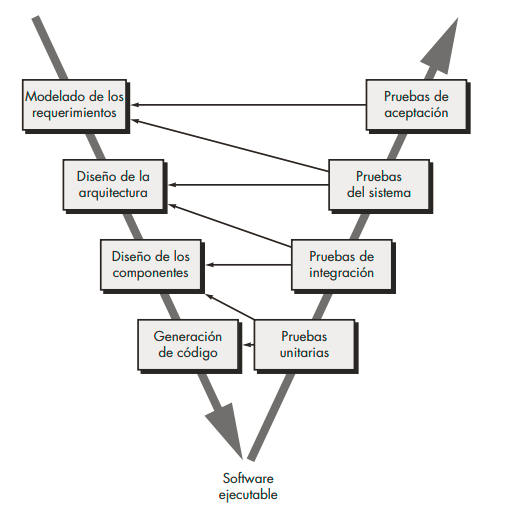
\includegraphics[scale=0.5]{image7.png}
  \caption{Modelo en cascada V. Extraída de \cite{pressmanIngenieriaSoftwareEnfoque2013}.}
  \label{fig:x modelo en v}
\end{figure}
%
\subsubsection{Ventajas}
\begin{itemize}
    \item Se adapta bien en proyectos con requerimientos claramente definidos.
    \item El proceso de validación genera un producto robusto.
\end{itemize}
\subsubsection{Desventajas}
\begin{itemize}
    \item Al igual que el método en cascada, es muy resistente al cambio de requerimientos.
    \item El proceso de validación no se realiza hasta que el software esté completado.
\end{itemize}

\section{Modelos incrementales}
\par En ciertos proyectos, el alcance del software es muy grande para desarrollarse de forma lineal. También puede suceder que es necesario entregar un software funcional en un corto plazo \cite{pressmanIngenieriaSoftwareEnfoque2013}. Para estos casos se pueden utilizar los modelos incrementales.
\par En este tipo de modelos, el software se avanza a partir de entregas incrementales, donde cada incremento suma nuevas funcionalidades. Generalmente, las primeras entregas incluyen los requerimientos urgentes, de forma que el cliente pueda validarlos en una etapa temprana del desarrollo \cite{sommervilleIngenieriaSoftware9a2011,pressmanIngenieriaSoftwareEnfoque2013}.
\par Cada uno de estos incrementos sigue el ciclo de vida en cascada, es decir que el desarrollo de una iteración se separa en módulos que deben ser terminados para avanzar al siguiente \cite{gujarathiSpiralDevelopmentNonSoftware2024}.
%
\begin{figure}[h]
  \centering
  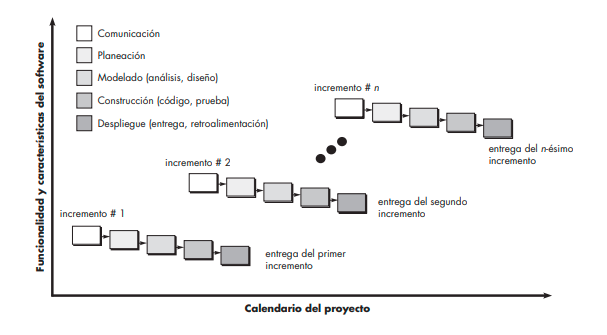
\includegraphics[scale=0.8]{image5.png}
  \caption{Modelo incremental . Extraída de \cite{pressmanIngenieriaSoftwareEnfoque2013}.}
  \label{fig:x Modelo incremental}
\end{figure}
\par El desarrollo incremental es particularmente útil cuando no se dispone del personal para la implementación completa del producto. Un equipo pequeño puede crear una versión básica del proyecto, y escalar a medida que la empresa crece \cite{pressmanIngenieriaSoftwareEnfoque2013}. 
Sin embargo, ciertas desventajas aparecen con este tipo de metodologías. En un principio, es difícil medir el progreso de un proyecto cuando las entregas se crean en rápida sucesión. A esto se suma que la estructura del sistema tiende a degradarse con el paso del tiempo debido a la periodicidad de cambios \cite{sommervilleIngenieriaSoftware9a2011}.


\section{Modelos evolutivos}
\par El software evoluciona con el tiempo. Los requerimientos de negocio y producto se modifican conforme avanza el desarrollo, y los constantes cambios en el mercado hacen que sea muy difícil desarrollar un software en tiempo y forma. Para esto existen los modelos evolutivos, que están diseñados explícitamente para adaptarse a un producto evoluciona con el tiempo \cite{pressmanIngenieriaSoftwareEnfoque2013}. Los modelos evolutivos son iterativos. Están pensados para desarrollar versiones cada vez más completas del software
%
%
\subsection{Modelo en espiral}
\par El modelo en espiral se acopla la naturaleza iterativa de hacer prototipos con el aspecto más lineal y controlado de los métodos en cascada. El software se desarrolla en una serie de entregas evolutivas, donde en cada iteración se obtiene una versión más completa del software \cite{pressmanIngenieriaSoftwareEnfoque2013}.
\begin{figure}[H]
  \centering
  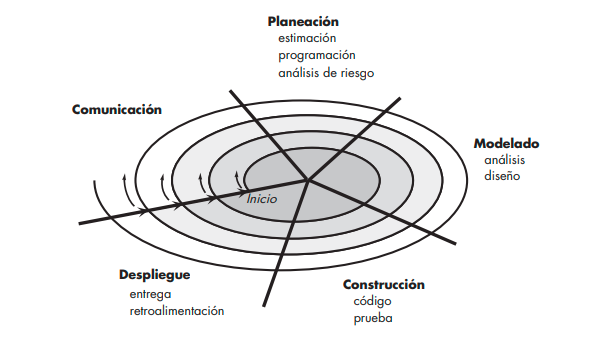
\includegraphics[scale=0.8]{image10.png}
  \caption{Modelo en espiral. Extraída de \cite{pressmanIngenieriaSoftwareEnfoque2013}.}
  \label{fig:x Modelo en espiral}
\end{figure}
\par El modelo en espiral se divide en un conjunto de actividades estructurales que se repiten en cada iteración. El primer circuito resulta en la especificación del producto. Las vueltas sucesivas se usan para desarrollar el prototipo y finalmente el resto de iteraciones son para crear el producto final \cite{pressmanIngenieriaSoftwareEnfoque2013}.

\section{Metodologías ágiles}
\par Las metodologías ágiles aparecen por la necesidad de una metodología flexible y capaz de adaptarse a los constantes cambios \cite{bartoszScrumVideoGames2023}. Estas metodologías se desarrollan en los años 90, y nacen de la frustración que las empresas percibían respecto a metodologías lineales \cite{sommervilleIngenieriaSoftware9a2011,pressmanIngenieriaSoftwareEnfoque2013}. 
El objetivo es que el equipo de desarrollo se enfoque en crear el software en vez de diseñar y documentar. Además, toman conceptos del desarrollo incremental, donde el producto se avanza generando iteraciones que son entregables a un cliente \cite{pressmanIngenieriaSoftwareEnfoque2013}.

\par Hay varias implementaciones de metodologías ágiles. Una de las más populares es Scrum, explicada en la sección a continuación.

\section{Scrum}
\par Tango Scrum como el resto de metodologías ágiles nacen de la necesidad de una metodología flexible y adaptable a los constantes cambios de los mercados tecnológicos \cite{bartoszScrumVideoGames2023}. Es una respuesta a las metodologías tradicionales, como Waterfall, las cuales priorizan seguir un plan definido \cite{cynthiachizobaekechiEnhancingAgileProduct2024}. En este sentido, Scrum representa un cambio de paradigma, que se enfoca en un sistema flexible, iterativo y colaborativo sobre el acercamiento basado en planes estrictos y documentación.
\par Scrum se basa en la idea de dividir el desarrollo de un software en pequeñas iteraciones llamadas sprints, generalmente durando un máximo de 4 semanas. El objetivo es que cada sprint produzca incrementalmente un producto usable, el cual puede ser presentado a un usuario final \cite{bartoszScrumVideoGames2023}.
\par Hoy en día, las empresas trabajan para crear productos digitales que satisfagan las necesidades de sus clientes, no sólo en videojuegos, si no que en la industria del software en general. Esto presenta un mayor desafío para una empresa pequeña, que aún debe competir en un mercado global a pesar de tener menos recursos \cite{putrianasariProblemsAdoptionAgileScrum2024}.Es por esto que muchas empresas implementan Scrum, una metodología que acepta el cambio constante y prepara a la institución para un ambiente dinámico y un futuro incierto \cite{putrianasariProblemsAdoptionAgileScrum2024}.
\par Scrum se basa en una serie de principios, donde los principales son:
\begin{itemize}
  \item Equipos autogestionados: a diferencia de otras metodologías, que siguen modelos jerárquicos, los equipos de Scrum tienen autoridad sobre su trabajo \cite{cynthiachizobaekechiEnhancingAgileProduct2024}. El objetivo es generar colaboración y responsabilidad por parte de los integrantes.
  \item Desarrollo iterativo: los proyectos que aplican Scrum se construyen en base a múltiples iteraciones del producto, mejorando la funcionalidad y calidad en cada una de ellas. El objetivo es motivar la adaptación continua de feedback, y la posibilidad de responder a cambios de manera rápida y efectiva \cite{cynthiachizobaekechiEnhancingAgileProduct2024}.
  \item Enfoque en el usuario final: con Scrum se busca involucrar al usuario en cada iteración del producto, de forma que esté alineado con las demandas del mercado \cite{cynthiachizobaekechiEnhancingAgileProduct2024}.
\end{itemize}
%
%
\subsection{Equipos}
\par En Scrum, el equipo consiste de 3 partes, el \emph{Scrum Master}, el \emph{Product Owner} y los \emph{Developers}. Todas las partes trabajan para cumplir un objetivo en común, llamado \emph{Product Goal} \cite{schwaberScrumGuide2020}. Además, se encuentra el rol de los \emph{Stakeholders}, que alinean al equipo a las demandas del mercado \cite{schwaberScrumGuide2020}.
\par Los equipos de Scrum son autogestionados, es decir que los miembros deciden en conjunto el itinerario de tareas, y las responsabilidades de cada uno. Se recomienda que el tamaño del equipo no supere las 10 personas, ya que de otra forma se complica la comunicación y la autonomía.
\subsubsection{Developers}
\par El equipo de \emph{Developers} se encarga de trabajar en cualquier aspecto de un \emph{Increment} en cada \emph{Sprint}. Sus tareas consisten en crear un plan para el \emph{Sprint}, llamado \emph{Sprint Backlog}, y llevarlo a cabo, considerando lo indicado por el \emph{Definition of Done}.
%
\subsubsection{Product Owner}
\par El \emph{Product Owner} se encarga de manejar el \emph{Product Backlog}. Este rol implica la creación, priorización y comunicación constante deeste mismo, asegurando que refleje las necesidades del cliente y los objetivos estratégicos del negocio.
\par Este rol suele ser ocupado por una sola persona, y puede representar las necesidades de varios \emph{Stakeholders}.
%
\subsubsection{Scrum Master}
La tarea del \emph{Scrum Master} es establecer las prácticas de Scrum y asegurarse de que el equipo las cumpla. Su objetivo es facilitar la implementación de la metodología. Cabe destacar que no es un rol de liderazgo, si no que trabaja como facilitador, ayudando al equipo a resolver impedimentos y mejorar su rendimiento.
\subsubsection{Stakeholders}
\par Se considera un \emph{stakeholder} a cualquier entidad que esté interesada en el éxito del producto. Ejemplos de \emph{stakeholders} son:
\begin{itemize}
  \item Clientes y usuarios finales
  \item Inversores
  \item Proveedores y vendedores
\end{itemize}
%
%
\subsection{Eventos}
\par Scrum busca promover una cultura de mejora continua, donde el equipo pueda aprender de sus experiencias y mejorar a futuro \cite{excelgchukwurahELEVATINGTEAMPERFORMANCE2024}. Es por esto que se establecen varios eventos que ayudan al equipo a mantenerse enfocado y en constante evolución.
%
\subsubsection{Sprints}
\par Las tareas del equipo se dividen en pequeñas iteraciones llamadas \emph{sprints}, generalmente durando un máximo de 4 semanas. El objetivo es que cada sprint produzca incrementalmente un producto usable, el cual puede ser presentado a un \emph{stakeholder} \cite{bartoszScrumVideoGames2023}.
\par Durante un \emph{Sprint} no pueden realizarse cambios a las tareas. El scope del próximo \emph{Sprint} puede ser renegociado en base a lo aprendido en el actual. Sólo un \emph{Product Owner} puede cancelar un \emph{Sprint}, en caso de que sea necesario.
%
\subsubsection{Sprint Planning}
\par Evento que inicia el \emph{Sprint}, donde se decide el trabajo que se realizará en este mismo. Este plan es creado por el \emph{Scrum Team}. El \emph{Product Owner} debe asegurarse que los miembros del equipo estén preparados para discutir los ítems más importantes del \emph{Product Backlog}. Los objetivos del \emph{Sprint planning} son:
\begin{itemize}
  \item Definir el \emph{Sprint Goal}.
  \item Seleccionar los ítems del \emph{Product Backlog} que se trabajarán durante el \emph{Sprint}.
  \item Desglosar las tareas seleccionadas del \emph{Product Backlog} en ítems pequeños, que no tomen más de un día de trabajo. Esto es llevado a cabo exclusivamente por los \emph{Developers}.
\end{itemize}
%
\subsubsection{Daily Scrum}
Reuniones diarias de 15 minutos donde los \emph{Developers} inspeccionan el trabajo del \emph{Sprint} y lo ajustan en caso de ser necesario. Cada desarrollador comparte su progreso y las tareas que realizará ese día \cite{bartoszScrumVideoGames2023,schwaberScrumGuide2020}.
%
\subsubsection{Sprint Review}
En este evento, el \emph{Scrum Team} presenta los resultados del \emph{Sprint} a los \emph{stakeholders}. Luego, se revisa qué se completó durante el \emph{Sprint}, y se evalúa si la dirección en la que se está trabajando cumple el \emph{Product Goal}.
%
\subsubsection{Sprint Retrospective}
Evento final que concluye el \emph{Sprint}. El \emph{Scrum Team} evalúa el progreso del mismo, investigando procesos, herramientas y el trabajo realizado. También se discute los aspectos positivos y negativos del \emph{Sprint}, y se encuentran formas de mejorar sobre las dificultades encontradas.
%
%
\subsection{Artefactos}
%
\subsubsection{Product Backlog}
\par Lista ordenada de tareas necesarias para llevar a cabo un producto. Representa el trabajo llevado a cabo por el \emph{Scrum Team}. Esta lista es constantemente refinada por el \emph{Product Owner} \cite{cynthiachizobaekechiEnhancingAgileProduct2024}, añadiendo detalles a las tareas, separándolas en ítems más precisos o cambiando el orden y prioridad.
\par El objetivo de este artefacto es asegurarse que el equipo se enfoque en las tareas más importantes, que generen la mayor cantidad de valor para el usuario final \cite{cynthiachizobaekechiEnhancingAgileProduct2024}.
%
\subsubsection{Product Goal}
\par Primero, se define a un producto como un objeto que produce valor para un usuario final \cite{schwaberScrumGuide2020}. Se considera entonces un \emph{Product Goal} al objetivo final que el \emph{Scrum Team} planea llevar a cabo. Es el objetivo a largo plazo del equipo.
%
\subsubsection{Sprint Backlog}
\par Set de ítems del \emph{Product Backlog} que se espera completar durante el \emph{Sprint}. Es creado y mantenido por los \emph{Developers}.
%
\subsubsection{Sprint Goal}
Objetivo del \emph{Sprint actual}, creado en el \emph{Sprint Planning}. Las tareas del \emph{Sprint Backlog} se deciden en torno a esta meta.
%
\subsubsection{Increment}
\par Artefacto que representa un paso hacia el \emph{Product Goal}. Son aditivos, es decir que se construyen en base a \emph{Increments} anteriores. Se presentan durante el \emph{Sprint Review} como evidencia empírica del trabajo realizado.
\par Los incrementos se crean cuando un ítem del \emph{Product Backlog} cumple el \emph{Definition of Done}.
%
\subsubsection{Definition of Done}
Este artefacto describe los estándares de calidad a los que debe llegar el trabajo actual para ser considerado un \emph{Increment}.
%
%
\subsection{Dificultades de Scrum}
\subsubsection{En el software tradicional}
\par Si bien varias organizaciones han sido impactadas positivamente por la implementación de Scrum, otras se han encontrado con dificultades. En 2020 se realizó una investigación que estima que la metodología falló en el 84\% de compañías pequeñas-medianas que lo implementaron \cite{putrianasariProblemsAdoptionAgileScrum2024}.
\par Putrianasari et al. \cite{putrianasariProblemsAdoptionAgileScrum2024} menciona 4 áreas en las que las compañías fallan a la hora de implementar Scrum.
\bigbreak
{\setlength{\parindent}{0cm}Manejo de personal}
\bigbreak
\par Una de las principales problemáticas es la falta de colaboración y comunicación en los equipos. Los desarrolladores tienden a enfocarse en sus objetivos individuales y pierden de vista los objetivos de la organización. Además, al tratarse de empresas pequeñas-medianas, los empleados rotan entre varios proyectos, cambiando constantemente de equipo. Esto va en contra de uno de los pilares de Scrum, donde el equipo debe ser autónomo, decidiendo sus tareas y evaluando su propio progreso \cite{putrianasariProblemsAdoptionAgileScrum2024}.
\bigbreak
\par Por otro lado, la resistencia al cambio por parte de los empleados puede traer problemas a la hora de implementar Scrum eficientemente. Esto viene de la falta de conocimiento de la metodología, un equipo de tamaño incorrecto, o de la falta de compromiso por parte de los trabajadores \cite{putrianasariProblemsAdoptionAgileScrum2024}.
\bigbreak
{\setlength{\parindent}{0cm}Proceso de adopción}
\bigbreak
\par Varias dificultades pueden aparecer a la hora de llevar a cabo la implementación. Una de ellas, la falta de comprensión de los conceptos y principios de Scrum. La investigación nota que algunas organizaciones ven el éxito que la metodología trae a otras empresas y se apresuran a implementarlo sin analizar cómo ayudaría en sus procesos de desarrollo.
\bigbreak
{\setlength{\parindent}{0cm}Problemas organizaciones}
\bigbreak
\par Para implementar Scrum exitosamente, las empresas deben dar una definición de éxito y alinear las prácticas de Scrum con los objetivos de la organización. Al fallar en alguno de estos procesos, la metodología no puede ser aplicada correctamente.
\bigbreak
{\setlength{\parindent}{0cm}Problemas técnicos}
\bigbreak
\par En algunos casos se nota que las empresas no utilizan herramientas y tecnología que facilitan la implementación de Scrum. Además, se observan casos donde el presupuesto prestado para establecer la metodología no cubre estas tecnologías.
%
\subsubsection{Scrum-but}
\par Si bien la guía de Scrum dictamina que se deben evitar cambios a sus estructuras \cite{schwaberScrumGuide2020}, las prácticas de esta metodología rara vez son seguidas de forma consistente \cite{HawaiiInternationalConference2020}. Es común ver implementaciones parciales de Scrum, donde sólo se aplican ciertos eventos o artefactos.
Hassani-Alaoui et al. \cite{HawaiiInternationalConference2020} identifica 3 situaciones donde el éxito de un proyecto se ve afectado por desviar de las prácticas de Scrum:
\begin{enumerate}
    \item La calidad del producto se ve afectada cuando un equipo no es autónomo. idealmente, los miembros del equipo se encargan de planear el sprint. Sin embargo, hay ocasiones donde esta responsabilidad pasa al Product Owner, Scrum Master, o alguna posición de manager similar. Esta pérdida de control se puede traducir en estimaciones incorrectas y por lo tanto una mala performance del equipo.
    \item El product owner debe ser el único responsable de manejar el product backlog. Cuando el product owner no es capaz de organizar y planear el backlog, el equipo no es capaz de trabajar en los ítems que el cliente desea priorizar.
    \item Las retrospectives son importantes para tener un paso de reflexión y mejora de los procesos de trabajo. En los casos donde esta reunión no se realizaba, o se utilizaba para expresar frustraciones en vez de buscar soluciones para ellas, se pudo observar una pérdida de eficiencia y efectividad.
\end{enumerate}
\par Por otro lado, Ramirez Lathi et.al \cite{lahtiScrumButIndicatorProcess2022} encuentra una relación entre anti-patrones a la hora de desarrollar un software y la aplicación de Scrum-but. Su investigación muestra cómo una empresa que evita algunos de los artefactos importantes, como Sprints o Testing, genera código que es propenso a errores y deuda técnica.


\section{Kanban}
\par Ideado por Taiichi Ohno en 1953, Kanban es un framework visual comúnmente utilizado para implementar metodologías ágiles \cite{tettehEmpiricalStudyAgile2024,montegalianoImplantarScrumCon2016}. El sistema consiste en dividir las tareas en una serie de tarjetas visuales situadas en un tablero, el cual está dividido en columnas e indican su estado actual. 
\begin{figure}[H]
  \centering
  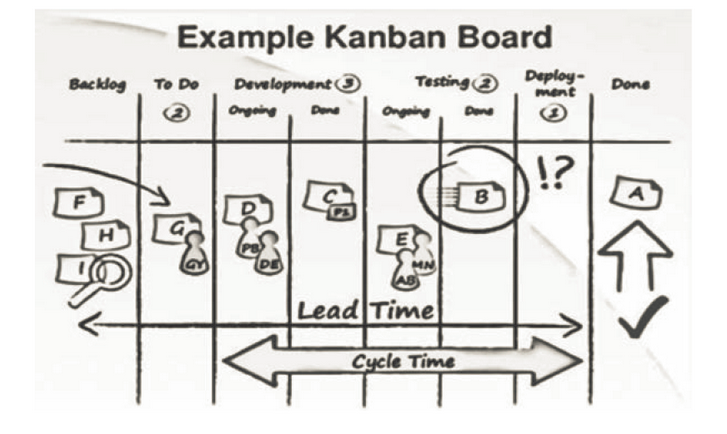
\includegraphics[scale=0.5]{image1.png}
  \caption{Ejemplo de un tablero de Kanban. Extraída de \cite{montegalianoImplantarScrumCon2016}}
  \label{fig:x Tablero kanban}
\end{figure}
\par Las tareas son representadas por tarjetas que avanzan por el tablero a medida que se actualiza su estado actual \cite{montegalianoImplantarScrumCon2016,canosaferreiroSCRUMTeoriaImplementacion2024}. El tablero de trabajo suele tener las siguientes columnas:
\begin{itemize}
    \item \textbf{TO DO}, que representa el trabajo que aún no se ha comenzado.
    \item \textbf{DOING}, que representa el trabajo que se está realizando actualmente.
    \item \textbf{DONE}, que representa el trabajo que se ha completado.
\end{itemize}
\par Este modelo establece una serie de prácticas a seguir:
\begin{itemize}
    \item \textbf{Flujo de trabajo visible}: Las tareas a realizar y el estado en que están son visibles para todos los participantes. Se puede implementar de forma física, utilizando una pared / pizarrón y post-its, o utilizar herramientas como Trello \cite{CaptureOrganizeTackle}. Aún así, es importante plasmar el sistema de forma visual \cite{montegalianoImplantarScrumCon2016,canosaferreiroSCRUMTeoriaImplementacion2024}.
    \item \textbf{Número limitado de tareas}: Para fomentar la agilidad, se limita la cantidad de tareas a realizar. Un miembro del equipo debería tener asignado un número pequeño de tareas en cada columna, de forma que pueda avanzar constantemente. En una situación ideal, un participante es capaz de terminar 1 o 2 tareas al día \cite{montegalianoImplantarScrumCon2016,canosaferreiroSCRUMTeoriaImplementacion2024}.
    \item \textbf{Medir el tiempo de trabajo}: Es importante hacer un seguimiento del avance de las tareas. Recopilar estas métricas permite mejorar los procesos de trabajo y abordar las posibles dificultades que aparezcan  \cite{montegalianoImplantarScrumCon2016,canosaferreiroSCRUMTeoriaImplementacion2024}. Algunas métricas comunes son “lead time”, “touch time” o velocidad, las cuales se estudian en otra sección del trabajo. 
    \item \textbf{Implementar políticas de procesos}: Es necesario establecer criterios que ayuden a mantener un buen ambiente de desarrollo \cite{canosaferreiroSCRUMTeoriaImplementacion2024}. Algunos de ellos pueden ser límite de tareas por personas o protocolos para decidir si una tarea puede ser cancelada o pospuesta. 
\end{itemize}


\section{Métricas}
\par Una forma de observar el progreso de un proyecto es recolectando información sobre las tareas que realizan los developers, y observar si aparecen patrones que indiquen la eficiencia del trabajo realizado. A continuación, se nombran algunas de las métricas comúnmente estudiadas.
%
\subsubsection{Lead Time}
\par Registra el tiempo que toma una tarea, desde que se extrae del Product Backlog hasta que es finalmente entregado. Sirve para estimar tiempos de entrega, medido en días \cite{gaeteEnfoqueAplicacionAgil2021}.
%
\subsubsection{Touch Time}
Registra el tiempo real que toma finalizar una tarea, descontando los posibles periodos de inactividad. Se mide en horas de trabajo \cite{gaeteEnfoqueAplicacionAgil2021}.
%
\subsubsection{Velocidad}
Cantidad de ítems de trabajo completados en cada iteración. Mide la productividad del equipo, y busca maximizar el número de requisitos terminados \cite{gaeteEnfoqueAplicacionAgil2021}.
%
\subsubsection{Requisitos no completados}
Registra la cantidad de requisitos que no se completaron durante la iteración a pesar de haberse establecido como uno \cite{gaeteEnfoqueAplicacionAgil2021}.


\printbibliography
\end{document}